\subsection{Felsorolások}

%
\begin{frame}
  \begin{description}[m]
    \item[\texttt{list-style-type}] \hfill \\ Felsorolásjel típusa\\
    \begin{itemize}
      \item Számozott listákhoz, pl. \texttt{decimal} (arab számok), \texttt{lower-alpha} (kisbetűk), \texttt{upper-roman} (római számok nagybetűkkel)
      \item Nem számozott listákhoz, pl. \texttt{disc} (körlemez), \texttt{circle} (körvonal), \texttt{square} (négyzet)
      \item Eltüntetés: \texttt{none}
    \end{itemize}
  \end{description}
\end{frame}

%
\begin{frame}
  \begin{columns}[c]
    \column{0.45\textwidth}
      \begin{exampleblock}{\textattachfile{szamozott.html}{szamozott.html}}
        \begin{center}
          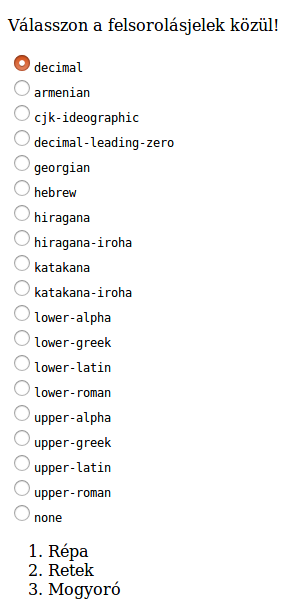
\includegraphics[width=.37\textwidth]{szamozott.png}
        \end{center}
      \end{exampleblock}
    \column{0.45\textwidth}
      \begin{exampleblock}{\textattachfile{nemszamozott.html}{nemszamozott.html}}
        \begin{center}
          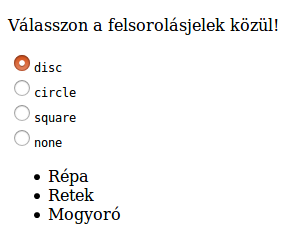
\includegraphics[width=.7\textwidth]{nemszamozott.png}
        \end{center}
      \end{exampleblock}
  \end{columns} 
\end{frame}

%
\begin{frame}
  \begin{columns}[c]
    \column{0.7\textwidth}
      \begin{description}[m]
        \item[\texttt{list-style-image}] \hfill \\ A felsorolásjel egy kép \texttt{url()} függvénnyel, vagy \texttt{none}.\\
        Érdemes megadni a \texttt{list-style-type}-ot is, hátha nem lehet megjeleníteni a képet.
      \end{description}
      \vfill
      \begin{exampleblock}{\textattachfile{sajatjelolo.html}{sajatjelolo.html}}
        \scriptsize
        \lstinputlisting[style=HTML,linerange={7-7},numbers=left,firstnumber=7]{sajatjelolo.html}
      \end{exampleblock}
    \column{0.25\textwidth}
      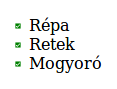
\includegraphics[width=\textwidth]{sajatjelolo.png}
  \end{columns} 
\end{frame}

%
\begin{frame}
  \begin{columns}[c]
    \column{0.7\textwidth}
      \begin{description}[m]
        \item[\texttt{list-style-position}] \hfill \\ A felsorolásjel helyzete\\
        \begin{itemize}
          \item \texttt{outside}: a bekezdés bal széle előtt, alapértelmezés.
          \item \texttt{inside}: a bekezdésen belül, a szöveg részeként.
        \end{itemize}
      \end{description}
      \vfill
      \begin{exampleblock}{\textattachfile{kivulbelul.html}{kivulbelul.html}}
        \scriptsize
        \lstinputlisting[style=HTML,linerange={7-9},numbers=left,firstnumber=7]{kivulbelul.html}
      \end{exampleblock}
    \column{0.25\textwidth}
      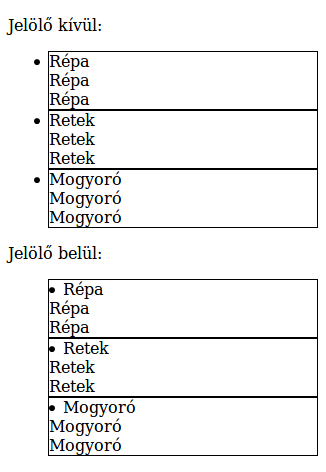
\includegraphics[width=\textwidth]{kivulbelul.png}
  \end{columns} 
\end{frame}

%
\begin{frame}
  Rövidítés:\\
  \begin{description}[m]
    \item[\texttt{list-style: list-style-type list-style-position list-style-image}] \hfill \\ Ha bármelyik hiányzik, az alapértelmezett értéket fogják használni.
  \end{description}
\end{frame}

%
\begin{frame}
  \begin{columns}[c]
    \column{0.55\textwidth}
      Készítse el a mellékelt ábrának megfelelő weboldalt! A felső rész felsorolásjeleként használja a \textattachfile{rouge.png}{rouge.png} fájlt!
    \column{0.4\textwidth}
      \begin{exampleblock}{\textattachfile{felsorolasok.html}{felsorolasok.html}}
        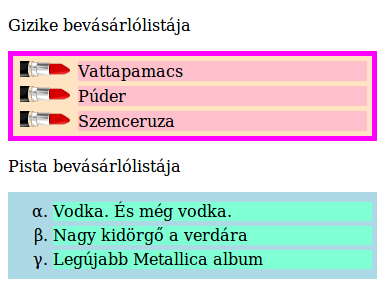
\includegraphics[width=\textwidth]{felsorolasok.png}
      \end{exampleblock}
  \end{columns} 
\end{frame}
